\documentclass ../main.tex]{subfiles}

\begin{document}



\vspace{3cm}
\chapter{Nociones Previas}

En el estudio de partículas elementales, notamos que experimentalmente se observan efectos tanto cuanticos como relativistas fenomenologicamente. Por lo que para trabajar con ellas se deberá tener en cuenta tanto la mécanica cuántica como la relatividad especial. La teoría con la que más nos acomodará trabajar será la \textbf{Teoría Cuantica de Campos (QFT)} pues tomará ambos efectos en consideración y nos permitirá estudiar eventos que sucedan a velocidades comparables con la velocidad de la luz $c$ en regiones pequeñas.\\

\begin{figure}[h] % "h" intenta colocar la imagen aquí
    \centering
    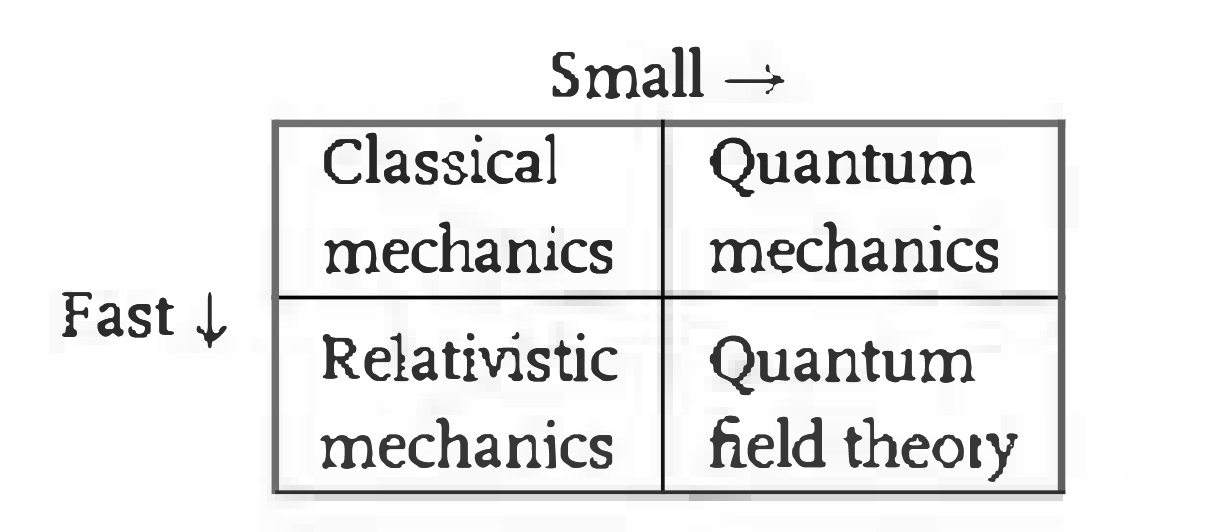
\includegraphics[width=0.5\textwidth]{img/Captura de pantalla 2025-03-29 000744.png}
    \label{fig:graf_QFT}
\end{figure}


Es por esto que para poder estudiar QFT se deberán tener nociones tanto de mécanica clásica como cuántica. En este apunte, no se considerarán los efectos del campo gravitacional. Como las interacciones a estudiar ocurren en regiones pequeñas, el efecto gravitacional será considerado despreciable. 

%quizas podríamos poner aca el decaimiento beta o otros ejemplos pero no sabia cuales poner pq no todos son d clasica 

\section{Primera clase}

\subsection{Derivación de las Ecuaciones de Euler-Lagrange}

Sea la acción $S[q(t)]$, donde $q(t)$ son las coordenadas generalizadas del sistema. 

\begin{equation}
    S[q(t)] = \int dt L(q, \dot{q})
\end{equation} 

Ahora, ¿Cómo cambia $S$ si $q(t)$ cambia un poco?\\

Sea $q(t)$ una función dependiente del tiempo, bien definida en el intervalo $t \in [t_1 , t_2]$. Donde los puntos $q(t_1)$ y $q(t_2)$ estarán fijos, de manera que aunque $q(t)$ cambie su valor en $t_1$ y $t_2$ no cambiara. Así, como se muestra en la figura [\textbf{citar}], si consideramos todos los caminos que puede tomar $q(t)$, diferenciados por una diferencia infinitesimal $\delta q = \Phi(t)$ que a su vez será dependiente del tiempo, se podrá variar la acción. 


[foto clasica de la invarianza d la acción]


\begin{align}
    \delta S &= S[q(t) + \phi(t)] - S[q(t)] \notag \\
    &= \int_{t_1}^{t_2}dt L(q(t) + \phi(t), \frac{d}{dt}\left(q + \Phi \right)) -\int_{t_1}^{t_2}dt L(q(t), \dot{q}(t)) \label{var-accion1}\\
\end{align}

Además, considerando que: 

\begin{equation}\label{ec_1}
    f(x +\epsilon_1, y + \epsilon_2) = f(x,y) + \frac{\partial f}{\partial x}\epsilon_1 + \frac{\partial f}{\partial y}\epsilon_2 + \mathcal{O}(\epsilon_1^2, \epsilon_2^2, \epsilon_1, \epsilon_2) 
\end{equation}

Por lo tanto, introduciendo \eqref{ec_1} con $f(x +\epsilon_1, y + \epsilon_2) = L(q(t) + \phi(t), \frac{d}{dt}\left(q + \Phi \right))$ en \eqref{var-accion1}.

\begin{align*}
    \delta S &=  \int_{t_1}^{t_2}dt \left( L(q(t),\dot{q}(t)) + \frac{\partial L}{\partial q}\Phi + \frac{\partial L}{\partial \dot{q}} \frac{d\Phi}{dt} \right) -  \int_{t_1}^{t_2}dt L(q(t), \dot{q}(t))\\ 
    &=  \int_{t_1}^{t_2}dt  \left(\frac{\partial L}{\partial q}\Phi + \frac{\partial L}{\partial \dot{q}} \frac{d\Phi}{dt} \right) \\
    &=  \int_{t_1}^{t_2}dt  \left(\frac{\partial L}{\partial q}\Phi + \frac{d}{dt}\left( \Phi \frac{\partial L}{\partial \dot{q}} \right) - \frac{d}{dt}\left( \frac{\partial L}{\partial \dot{q}} \right)\Phi \right) \\
    &=  \int_{t_1}^{t_2}dt \frac{d}{dt}\left( \Phi \frac{\partial L}{\partial \dot{q}} \right) + \int_{t_1}^{t_2}dt \Phi \left(\frac{\partial L}{\partial q}- \frac{d}{dt}\left( \frac{\partial L}{\partial \dot{q}} \right) \right) \\
    &= 0 + + \int_{t_1}^{t_2}dt \Phi \left(\frac{\partial L}{\partial q}- \frac{d}{dt}\left( \frac{\partial L}{\partial \dot{q}} \right) \right) \\
    \delta S &=\int_{t_1}^{t_2}dt \Phi \left(\frac{\partial L}{\partial q}- \frac{d}{dt}\left( \frac{\partial L}{\partial \dot{q}} \right) \right).\\
\end{align*}

Si se asume que el princiío de acción es estacionario $\delta S = 0$. Entonces: 

\begin{equation}
    \int_{t_1}^{t_2}dt \Phi \left(\frac{\partial L}{\partial q}- \frac{d}{dt}\left( \frac{\partial L}{\partial \dot{q}} \right) \right) = 0 \label{var-accion2}
\end{equation}

Finalmente, considerando a $f(t)$ arbitraria, en \eqref{var-accion2} el integrando de la integral deberá ser igual a cero. Por lo tanto, 

\begin{equation}
    \frac{\partial L}{\partial q} - \frac{d}{dt} \left( \frac{\partial L}{\partial \dot{q}} \right) = 0
\end{equation}


\subsection{Preguntas clase 1}
\subsubsection{Pregunta 1}
Escriba la ecuación de Schödinger para el àtomo de hidrógeno, incluyendo las contribuciones cinéticas tanto del protón como del electrón, además de la energía potencial de la interacción.
\\
\\
\textbf{Solución:}
\subsubsection{Pregunta 2}
Argumente que la formulación standard de la mecácnia cuántica no-relativista considera un número fijo de partículas y no permite describir transiciónes entre estados con número distinto de partículas. \\
\\
\textbf{Solución:}
\subsubsection{Pregunta 3}
Describa el efecto Compton y diga por qué razón el resultado clásico es distinto al observado. Calcule la longitud de Compton del electrón. \\
\\
\textbf{Solución:}
\subsubsection{Pregunta 4}
Describa el decaimiento beta ¿Cuál es la vida media de un neutrón? ¿Cómo interpreta tal número? \\
\\
\textbf{Solución:}
\subsubsection{Pregunta 5}
Deduzca las ecuaciones de Euler-Lagrange, argumentando cláramente cada uno de sus pasos. Explique porqué nunca es necesario preguntarse si la variación $\delta$ conmuta o no con la derivada temporal $\frac{d}{dt}$. Encuentre las ecuaciones de Euler-Lagrange para un Lagrangiano que dependec de un número arbitrario de coordenadas generalizadas $q_i(t)$ con $i=1,\dots ,N$. \\
\\
\textbf{Solución:}
Sea la acción
\begin{equation}
  S= \int_{t_1}^{t_2}dt L(\dot{q}^i,q^i,t) 
\end{equation}
Para lo cual $q^i(t)\quad , i=1,\dots , N$ son las coordenadas generalizadas las cuales están bien definidas en el intervalo de $t\in[t_1,t_2]$ en los cuales se tiene que las condiciones de borde homogéneas (shell) tal que, aunque las funcion pueda cambiar dentro del intervalo $(t_1,t_2)$ los valores en los extremos $t_1$ y $t_2$ no cambiará. Así, consideraremos una variacion del camino infinitesimal del camino que tomará, la cual denotaremos por $\delta q^i=\Phi^i(t)$ que al igual que las coordenadas, será dependiente del tiempo, la variación de la acción ante esta variacion infinitesimal de camino es denotada por
\begin{align*}
  \delta S & =S[q^i(t)+\Phi^i(t)]-S[q^i(t)] \\
           & = \int_{t_1}^{t_2} L\left[ q^i(t) + \Phi^i(t) , \frac{d}{dt}\left( q^i(t)+\Phi^i(t)\right ),t \right] - \int_{t_1}^{t_2}dtL (q^i(t), \dot{q}^i,t) 
\end{align*}
Ahora, se tiene la siguiente dependencia en el Lagrangiano  $L\left[ q^i(t) + \Phi^i(t) , \frac{d}{dt}\left( q^i(t)+\Phi^i(t)\right ),t \right]$ para lo cual se tomará una serie de Taylor con respecto al origen como sigue
\begin{align*} \label{taylor-L}
  L\left[q^i+\Phi^i, \frac{d}{dt}\left(q^i+ \Phi^i  \right) \right]= L + \partial_{q^i} L \; \Phi^i + \partial_{\dot{q}^i}L \;  \dot{\Phi} + \mathcal{O}({\Phi^i}^2,\dot{\Phi^i}^2 , \Phi^i, \dot{\Phi}^i)
\end{align*}
Con lo cual, si introducimos \eqref{taylor-L} sin tomar en cuenta los términos de $ \mathcal{O}({\Phi^i}^2,\dot{\Phi^i}^2 , \Phi^i, \dot{Phi}^i)$ se tiene lo siguiente
\begin{align*}
  \delta S  = \int_{t_1}^{t_2} dt \left(  L + \partial_{q^i} L \; \Phi^i + \partial_{\dot{q}^i}L \;  \dot{\Phi} \right) - \int_{t_1}^{t_2} L(q^i,\dot{q}^i,t)  
\end{align*}
Ahora, usando regla de Leibniz en el tercer término en la primera integral, se obtiene
\begin{align*} \label{leibniz}
  \frac{d}{dt}\left( \partial_{\dot{q}^i} L\; \Phi^i \right) & = \frac{d}{dt}\partial_{\dot{q}^i}\Phi^i + \partial_{\dot{q}^i}(L) \; \dot{\Phi}^i \\
  \frac{d}{dt}(\partial_{\dot{q}^i}L\;\Phi^i)  -\frac{d}{dt}( \partial_{\dot{q}^i}L)\; \Phi^i = & \partial_{\dot{q}^i}\dot{\Phi}^i
\end{align*}
Con lo cual, introduciendo \eqref{leinbiz} en el desarollo, obtenemos lo que sigue
\begin{align*}
  \delta S & = \int_{t_1}^{t_2} dt \left[  L + \partial_{q^i} L \; \Phi^i + \frac{d}{dt}(\partial_{\dot{q}^i}L \; \Phi^i)  -\frac{d}{dt} (\partial_{\dot{q}^i}L)\; \Phi^i\right] - \int_{t_1}^{t_2} L(q^i,\dot{q}^i,t)  \\
  & = \int_{t_1}^{t_2} dt \left[ L - L+ \partial_{\dot{q}^i} L \; \Phi^i - \frac{d}{dt}(\partial_{\dot{q}^i} L)\Phi^i\right]  + \int_{t_1}^{t_2}\frac{d}{dt}(\partial_{\dot{q}^i}L\; \Phi^i)
\end{align*}
Notese que el ùltimo término será igual a cero ya que este está evaluado en los los extremos, veamos que, por el teorema fundamental del cálculo:
\begin{equation*}
  \int_{t_1}^{t_2}dt \frac{d}{dt} (\partial_{\dot{q}^i}L \; \Phi^i) =  \left[\partial_{\dot{q}^i}L \; \Phi^i\right]_{t_1}^{t_2} = 0
\end{equation*}
Ya que, como sabemos $\Phi^i(t_1)=\Phi^i(t_2)=0$ son las condiciones de borde impuestas, así sigue que
\begin{align*}
  \delta S & = \int_{t_1}^{t_2} dt \left( \partial_{q^i}L + \frac{d}{dt}(\partial_{\dot{q}^i}L) \right)\Phi^i 
\end{align*}
Luego, se sume que el princpio de acción es estacionaro, con lo cual $S\delta \stackrel{!}{=}0$ con lo cual se obtiene
\begin{equation*}
  \delta S \stackrel{!}{=}0=\int_{t_1}^{t_2} dt \left( \partial_{q^i}L - \frac{d}{dt} (\partial_{\dot{q}^i}L) \right) \Phi^\i
\end{equation*}
Ahora, como se ha realizado para un intervalo de tiempos cualesquiera, entonces el integrando será cero para todo tiempo, lo cual es
\begin{align*}
  0 & =\left[\partial_{q^i}L-\frac{d}{dt}(\partial_{\dot{q^i}}L)\right] \Phi^i \\
  & = \partial_{q^i}L- \frac{d}{dt}(\partial_{\dot{q}^i}L)
\end{align*}
En donde se ha obviado el caso trivial en el cual $\Phi^i=0$ ya que esta es una función arbitraria. \\ 
Con lo cual, finalmente se llega a las ecuaciones de Euler-Lagrange para $q^i(t) \quad , i=1,\dots,N$ las cuale están dadas por
\begin{equation}
  \boxed{\partial_{q^i}L-\frac{d}{dt}(\partial_{\dot{q}^i}L)=0}
\end{equation}









\end{document}
